\chapter{А это что за штука? Устройство гитары}
\label{ch:guitar}

Гитара завоевала сердца многих благодаря простоте и изяществу своего устройства.

Гитара --- инструмент для извлечения звуков равномерно темперированного строя. Вспомним (см. раздел \ref{ch:music:tone}), что строй --- это правила отбора частоты колебаний основного тона для особых звуков, которые называются \emph{музыкальными}. Именно такие звуки извлекают из \emph{музыкального} инструмента.

Давайте увидим математику строя в конструкции гитары, а затем разберемся с тем, как правильно её на\emph{строить}.


\section{Может разберем? Конструкция}
\label{ch:guitar:construction}

Взглянем на рисунок \ref{fig:guitar:construction}, чтобы узнать, как называются отдельные части гитары.

\begin{figure}[!ht]
    \centering
    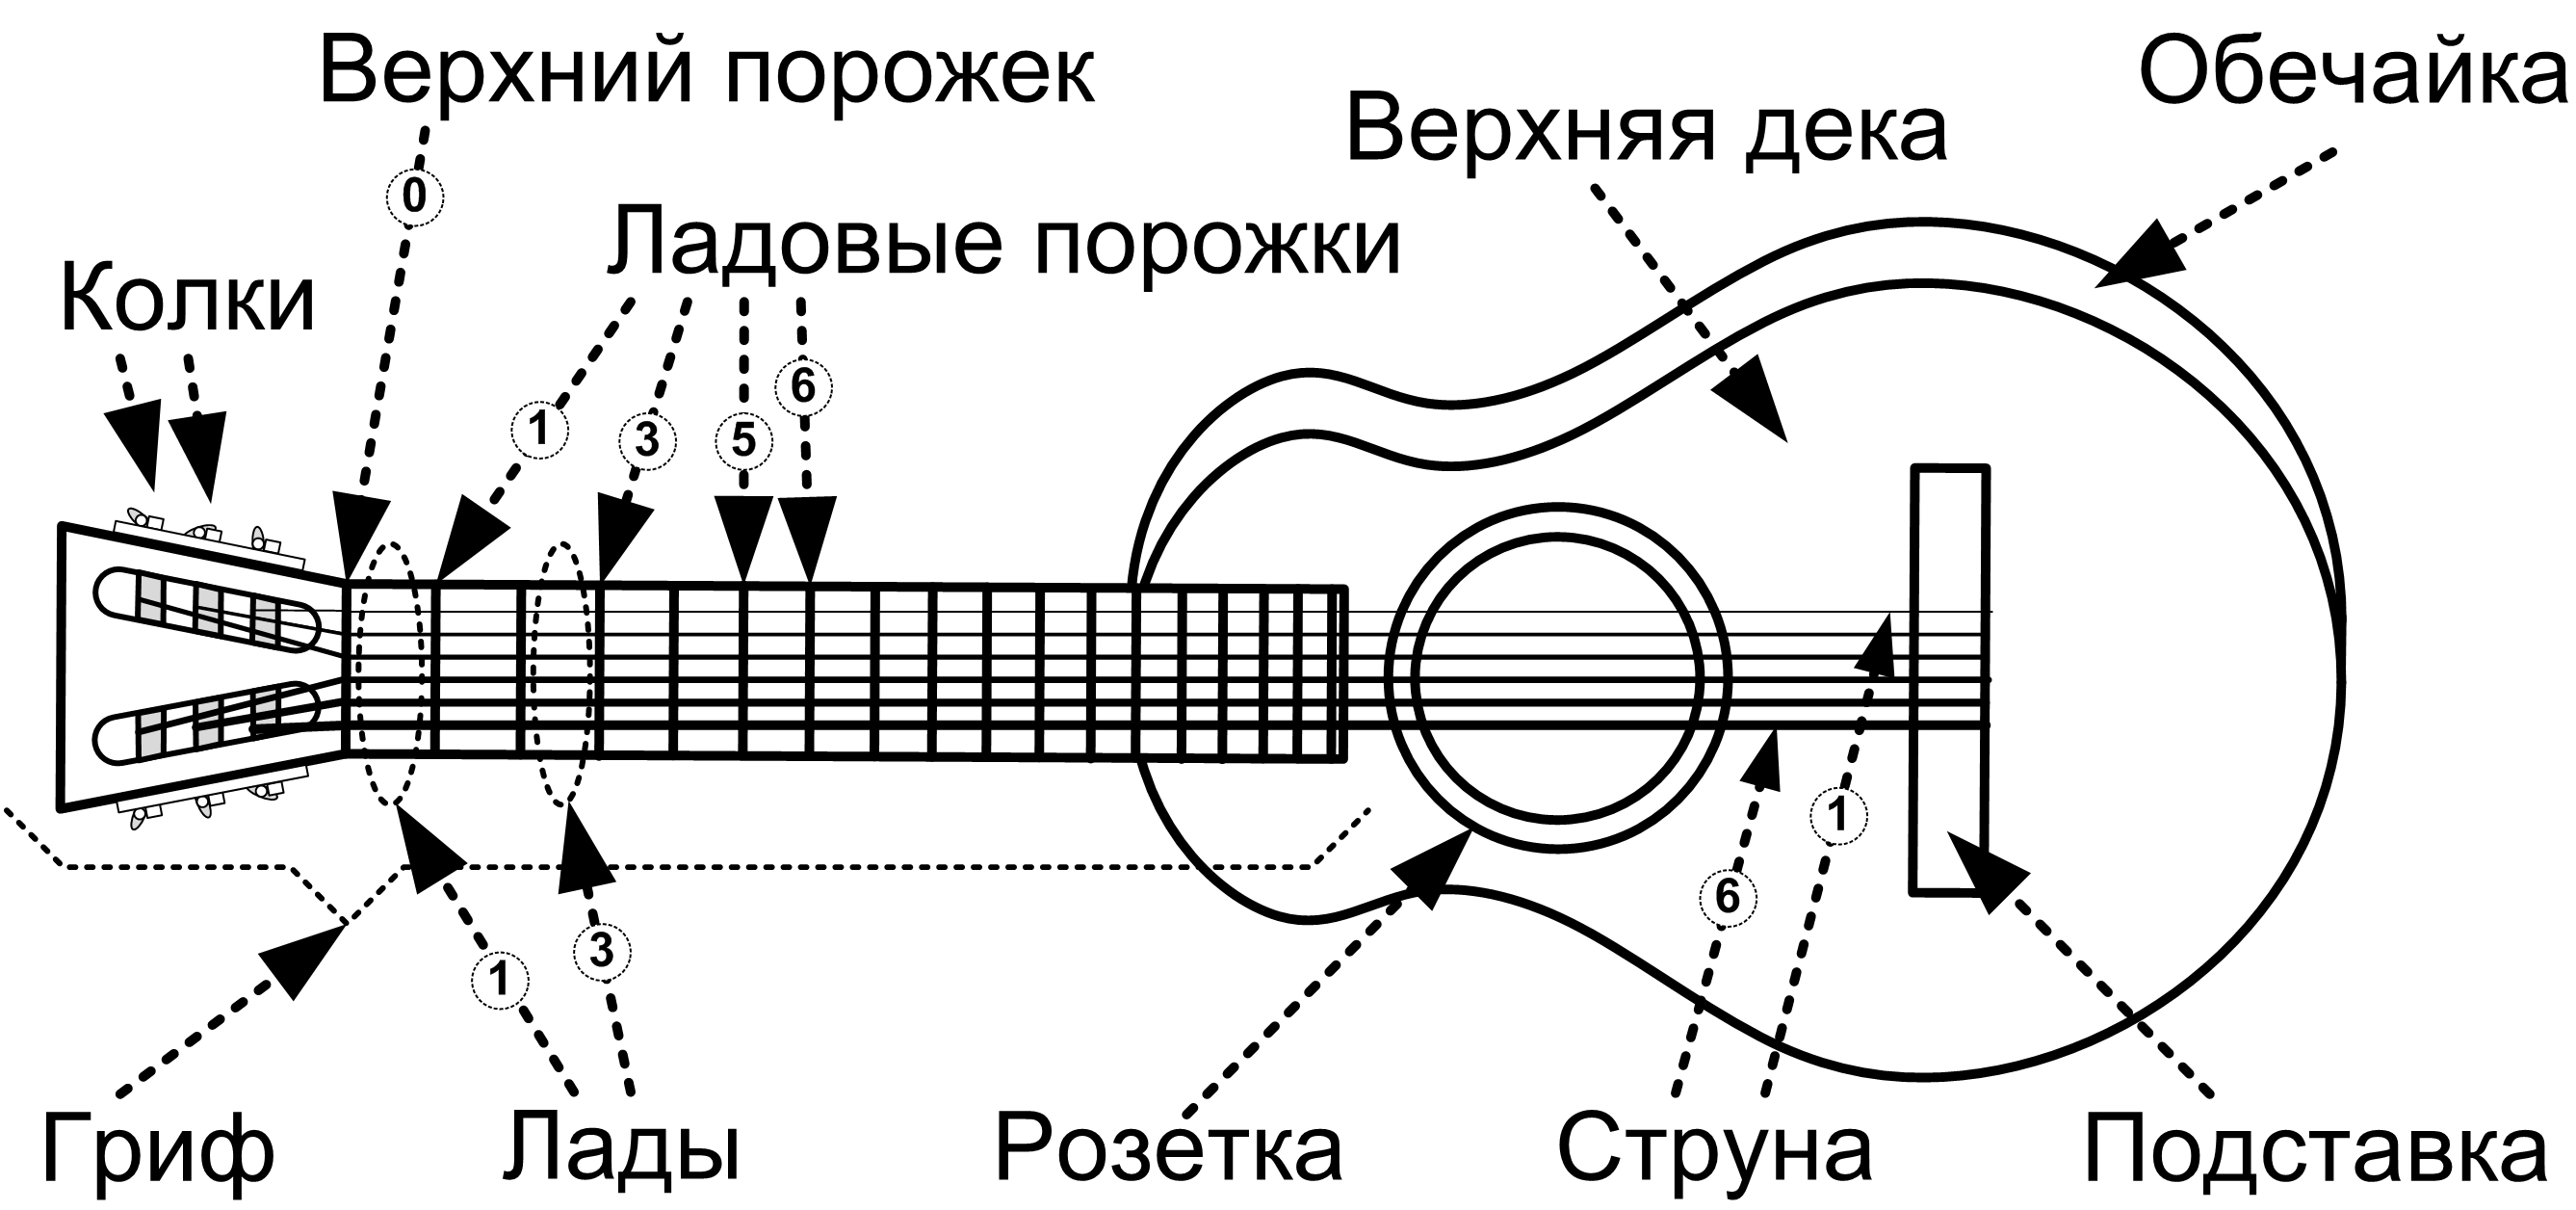
\includegraphics{fig/guitar-construction} 
    \caption{Устройство гитары}\label{fig:guitar:construction}
\end{figure} 

Отдельная \emph{струна} одним концом крепится к неподвижной \emph{подставке}, а вторым концом наматывается на барабанчик \emph{колка}. Червячный механизм колка позволяет очень тонко регулировать степень натяжения струны. Струна натягивается вдоль \emph{грифа}, поперек которого врезаны на определенном расстоянии друг от друга металлические выступы --- \emph{ладовые порожки}. Струна натянута так, что её звучащая (колеблющаяся) часть опирается своими концами на верхний порожек и на подставку соотвественно, а остальных ладовых порожков не касается, хотя и проходит достаточно близко к ним\footnote{
    Приведу все же немного справочных данных о расстояниях от струн до ладов. С одной стороны, чем оно меньше, тем легче и быстрее укорачивается струна, а с другой стороны, слишком <<зaниженная>> струна может во время игры начать звенеть, касаясь ладовых порожков. Для классической аккустической гитары (с нейлоновыми струнами) средние показатели такие: 
    \begin{itemize}
        \item расстояние от 1-й струны до 1-го ладового порожка составляет 0.61 мм, а до 12-го --- 3.18 мм;
        \item от 6-й струны до 1-го порожка --- 0.76 мм, а до 12-го --- 3.96 мм;
    \end{itemize}
    
    Для эстрадной аккустической гитары (со стальными струнами и анкерным стержнем внутри грифа) расстояния следующие:
    \begin{itemize}
        \item от 1-й струны до 1-го порожка --- 0.33 мм, а до 12-го --- 1.78 мм;
        \item от 6-й струны до 1-го порожка --- 0.58 мм, а до 12-го --- 2.29 мм;
    \end{itemize}
    
    Пусть вас не пугают приведенные с точностью до сотых долей миллиметра числа --- они являются расчетными. На практике регулировка осуществляется подтачиванием верхнего порожка и порожка на подставке. Замеры расстояния осуществляются (в порядке увеличения популярности): штангенциркулем, стальной слесарной линейкой, просто <<на глазок>> --- но никак не микрометром! У людей профессионально занимающихся доводкой гитар, обычно заготовлены пластинки нужной толщины, и высота контролируется простым просовыванием пластинки между струной и порожком.
    
    Единого стандарта на высоту струн нет. Профессионалы, естественно, занижают высоту струн до предела, чего новичкам делать не следует. С завода бюджетные гитары обычно поступают в магазины с <<завышенной>> высотой струн и требуют доводки. В хорошем музыкальном магазине либо <<доведут>> гитару при покупке, либо посоветуют гитарного мастера.
}

Известно, что частота колебаний струны зависит от степени её натяжения и её длины. Перед тем как играть, гитару \emph{настраивают}, то есть с помощью колков каждую струну натягивают так, чтобы она издавала строго определенный \emph{музыкальный} звук. Чем сильнее натянута струна, тем выше звук (т.е. тем больше частота колебаний струны). А уже играя, гитарист прижимает пальцем левой рукой струну к ладовому порожку, чем практически мгновенно укорачивает её звучащую часть. Что в свою очередь приводит к повышению звука, так как частота колебаний струны обратно пропорциональна её длине\footnote{Надо честно заметить, что частота колебаний струны зависит также и от силы её натяжения, которая меняется, когда струну <<зажимают>> на ладу. Но это влияние столь незначительно, что им можно пренебречь}. 

Теперь давайте вспомним о самых важных музыкальных единицах измерения расстояния между двумя \emph{музыкальными} звуками.
\begin{itemize}
    \item \emph{Октава} --- звук $x$ \emph{выше} звука $y$ на \emph{октаву}, если частота колебаний основного тона звука $x$ больше частоты основного тона звука $y$ вдвое. Чтобы повысить звук открытой струны на октаву, нужно укоротить её вдвое, сохранив натяжение.
    
    \item \emph{Полутон} --- двенадцатая часть октавы. Теоретически неделимое расстояние между двумя музыкальными звуками. Звук $x$ \emph{выше} звука $y$ на \emph{полутон}, если частота основного тона звука $x$ больше частоты основного тона $y$ в $\sqrt[12]{2}$. Откуда квадратные корни? Проверьте: двенадцать раз повысив высоту звука $y$ на полутон, получим звук $x$ с частотой в $(\sqrt[12]{2})^{12}$ больше частоты исходного $y$. Так как $(\sqrt[12]{2})^{12} = 2$, то мы получили расстояние в октаву, что и требовалось! 
\end{itemize}


\begin{Definition}[Суть гитарной простоты]
    Номер лада на грифе гитары соответствует количеству \emph{полутонов}, на которое \emph{повышается} звук открытой струны, если её зажать на этом ладу.
\end{Definition}

Сдвинулись по грифу на лад --- повысили (или понизили) звук на \emph{полутон}. Сдвинулись на 12 ладов --- повысили/понизили на \emph{октаву}. И вообще: над 12 ладовым порожком находится середина струны!

В соотвествии с правилами равномерно темперированного строя (см. раздел \eqref{ch:music:tone}) частота основного тона струны зажатой на $n$-м ладу $f(n)$ будет определяться как 
\[
    f(n) = f_\text{откр}\cdot(\sqrt[12]{2})^n,
\] 
где $f_\text{откр}$ --- частота основного тона открытой струны. А так как частота колебаний струны обратно-пропорциональна её длине, то длина зажатой на $n$-м ладу струны $L(n)$, дающей звук нужной частоты, будет определяться так:

\begin{equation}
    \label{eq:guitar:construction:length}
    L(n) = \frac{L}{(\sqrt[12]{2})^n},
\end{equation}
где $n$ --- номер лада ($0$-й лад соответствует открытой струне, см. рисунок \ref{fig:guitar:construction}), а $L$ --- общая длина <<открытой>> струны: от подставки до верхнего порожка.

\begin{figure}[!ht]
    \centering
    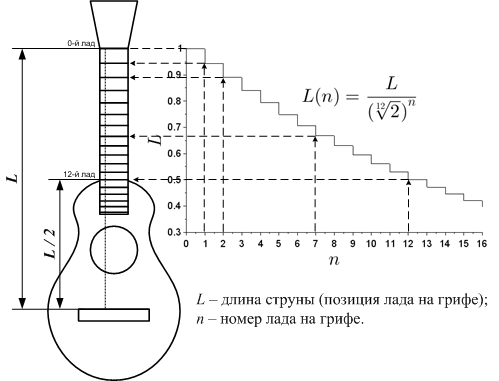
\includegraphics{fig/string-length.png}
    \caption{Расстояние между ладами}\label{fig:guitar:construction:length}
\end{figure} 

Вот и готова конструкция гитары! На рисунке \ref{fig:guitar:construction:length} соотнесён график функции \ref{eq:guitar:construction:length} с расположением ладов на гитарном грифе. Теперь ясно, например, почему по мере приближения к розетке расстояние между ладами становится все меньше.

Кстати, некоторые ушастые выпендрёжники говорят, что различают своим сверхмузыкальным слухом больше 12 нот в октаве! Давайте делить полутон! Есть спрос --- есть предложение: на некоторых гитарах можно заметить дополнительные ладовые порожки между <<каноническими>>, которые позволяют <<всунуть>> дополнительную ноту.

Играя, гитарист лишь меняет длину звучащего участка струны, зажимая струны на ладах. Однако редкие психи/мастера крутят колок во время исполнения, добиваясь сомнительных/удивительных музыкальных эффектов.


\section{Правильно устроена? --- не значит что настроена!}
\label{ch:guitar:tuning}


%TODO --- отсылка на ноты, удобно строить аккорды. Рисунки, расположение нот на грифе гитары. Расшифровка нетривиальных рисунков. Тонкости настройки. Резонанс. Проверка ногтем.

\begin{figure}[!ht]
    \centering
    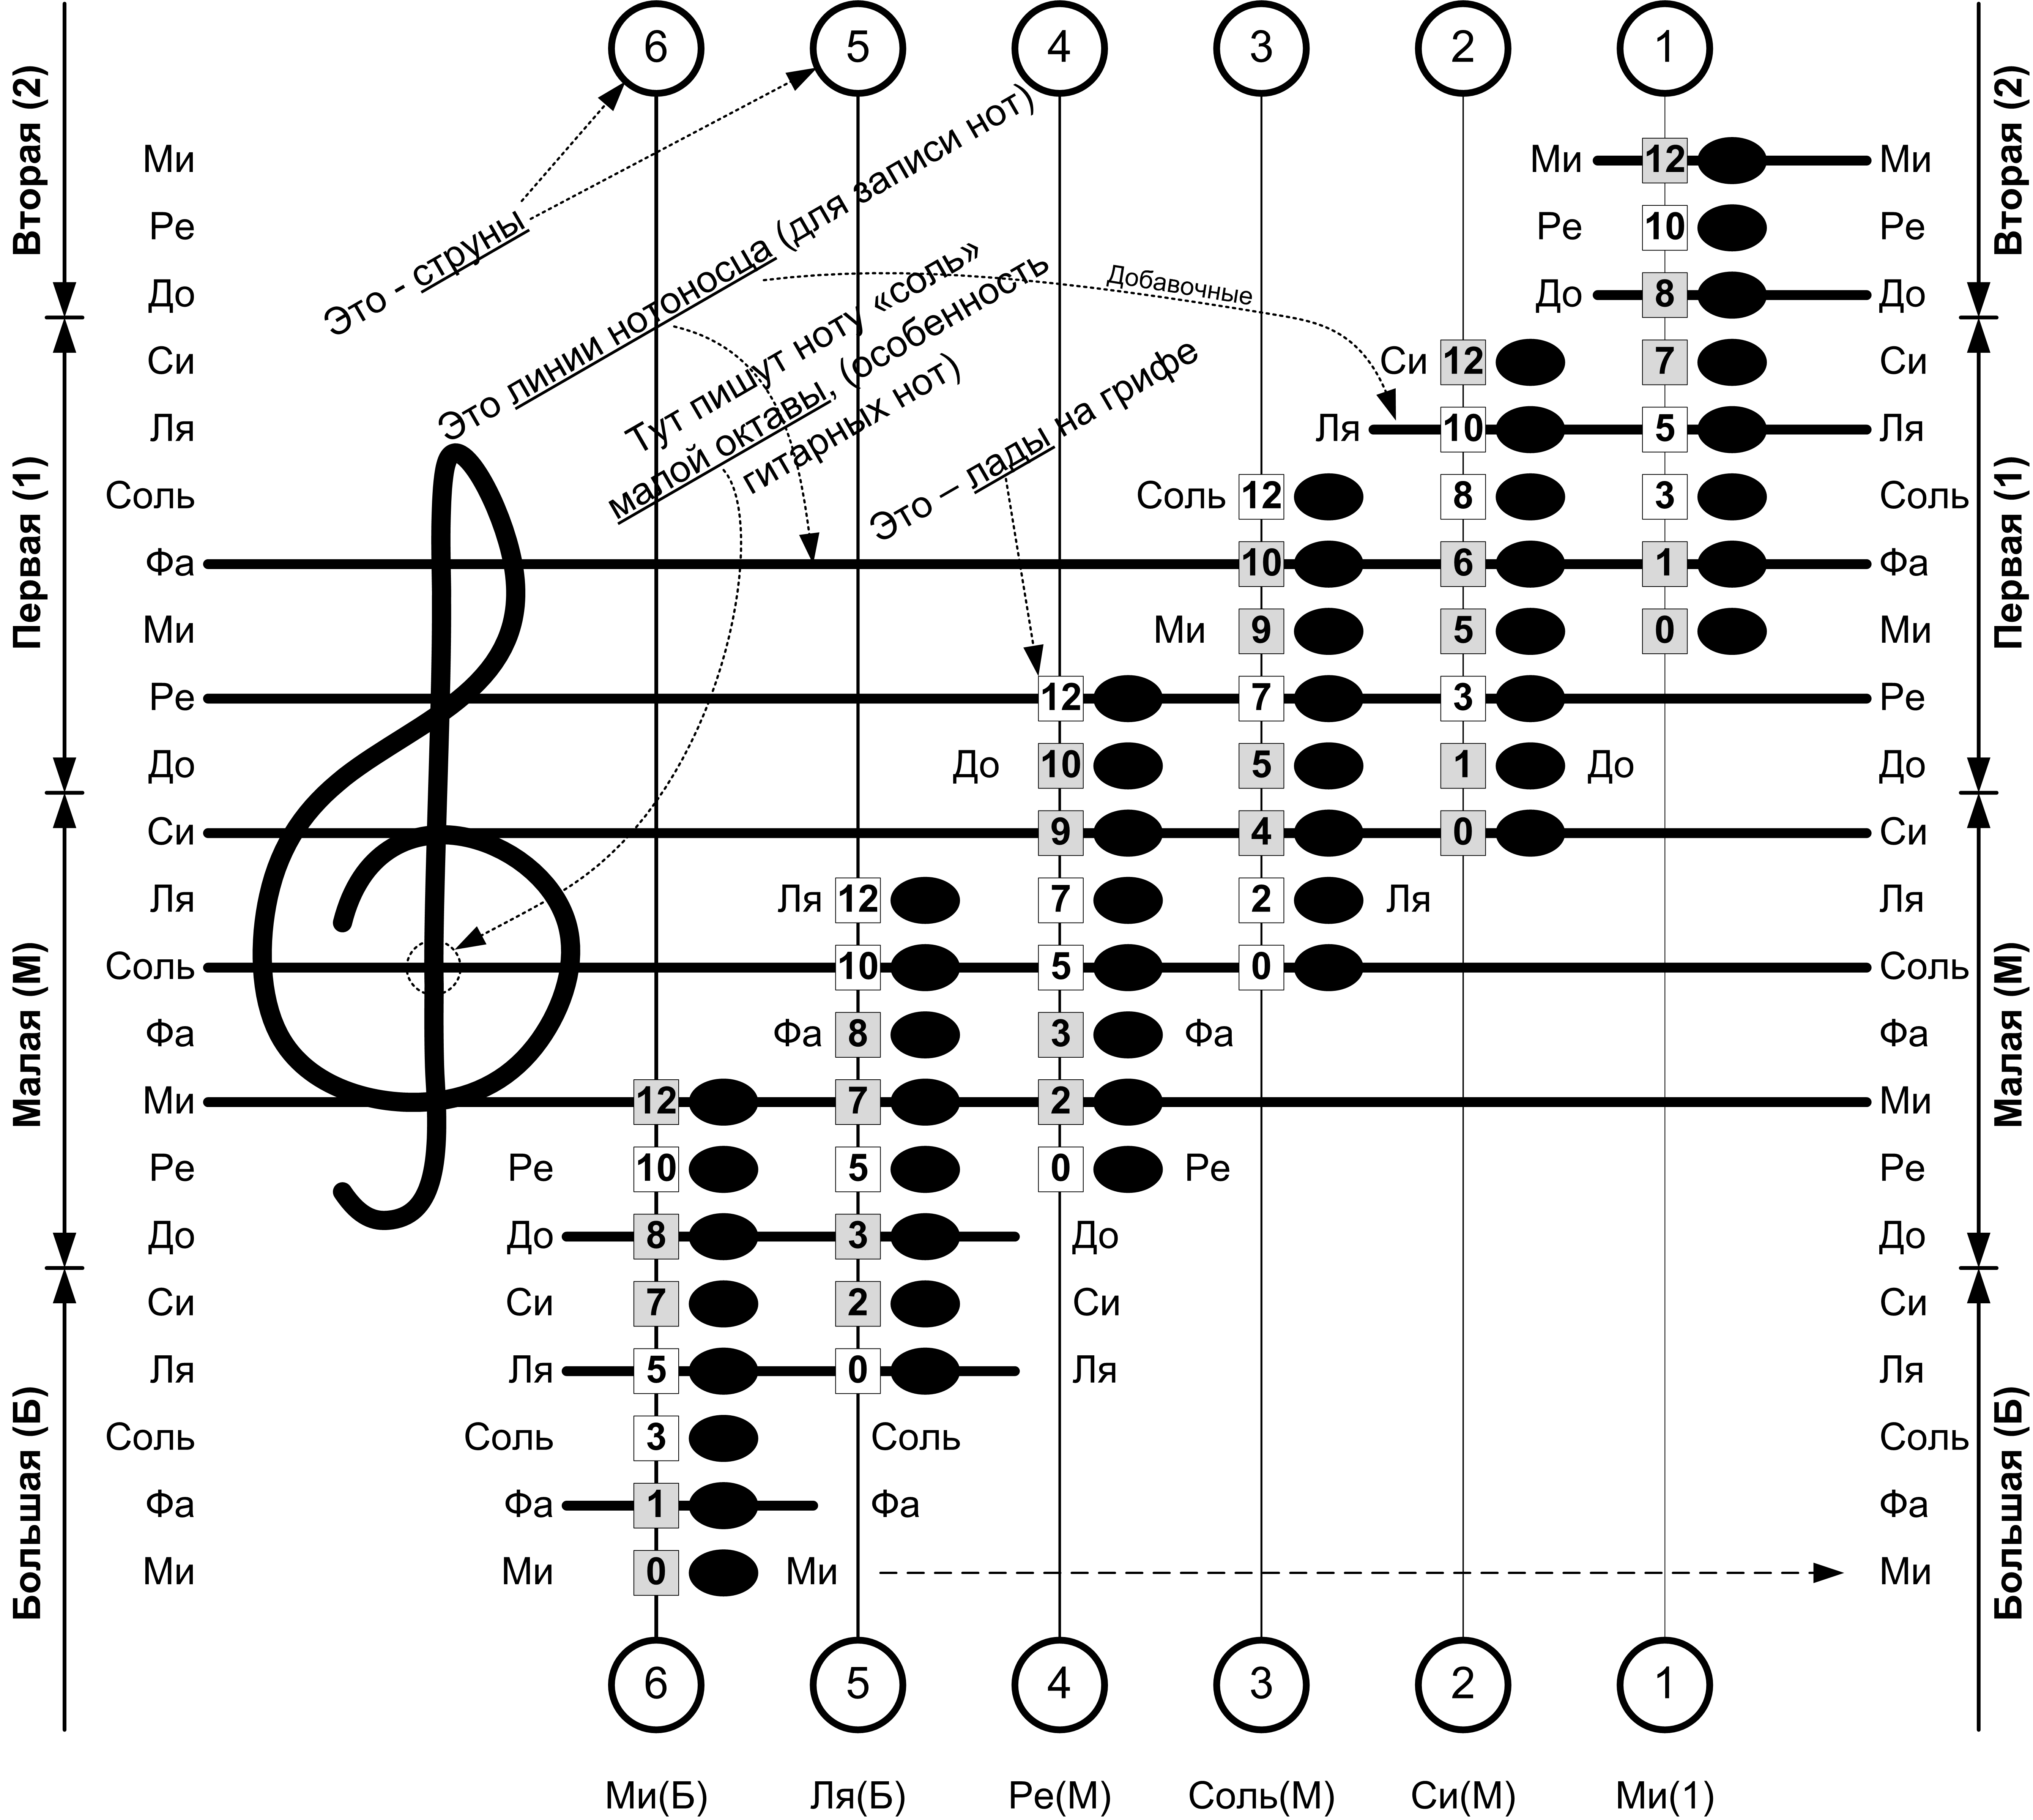
\includegraphics[width=\textwidth]{fig/lad-by-notes} 
    \caption{Ноты на грифе (гриф поперек нотоносца)}\label{fig:guitar:lad-by-notes}
\end{figure} 

\begin{figure}[!ht]
    \centering
    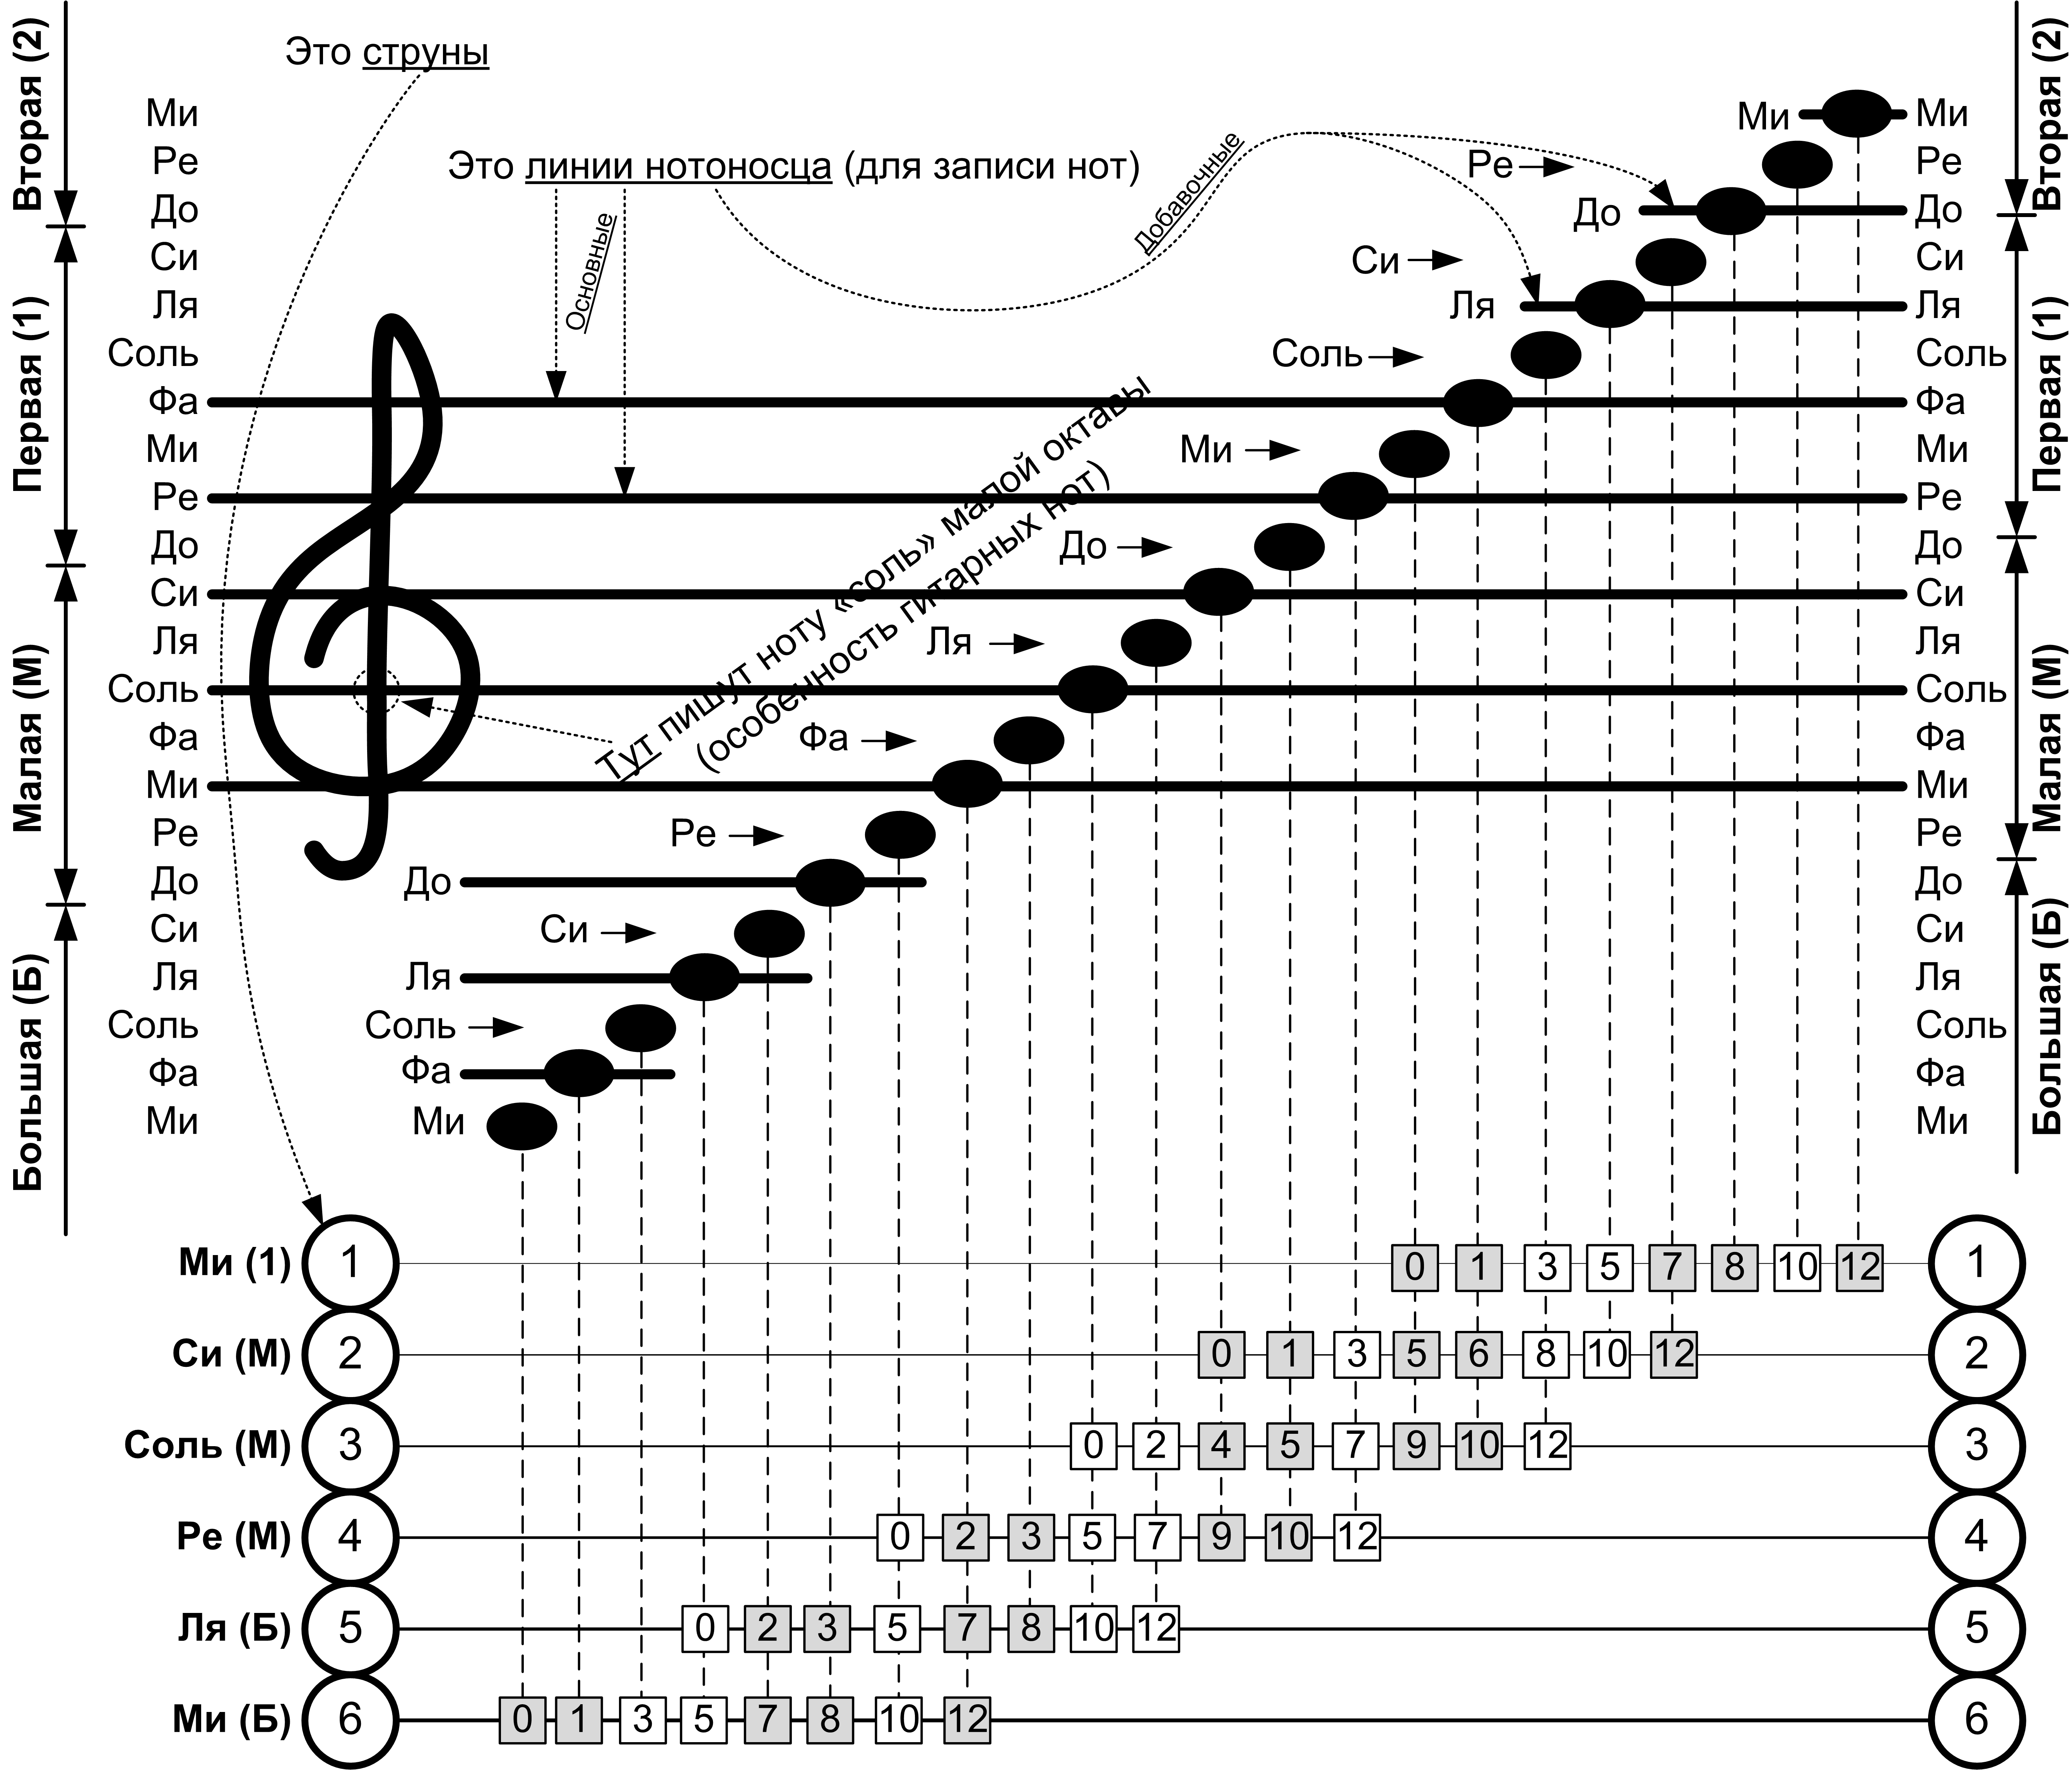
\includegraphics[width=\textwidth]{fig/lad-by-griph} 
    \caption{Ноты на грифе (гриф вдоль нотоносца)}\label{fig:guitar:lad-by-griph}
\end{figure} 

\begin{figure}[!ht]
    \centering
    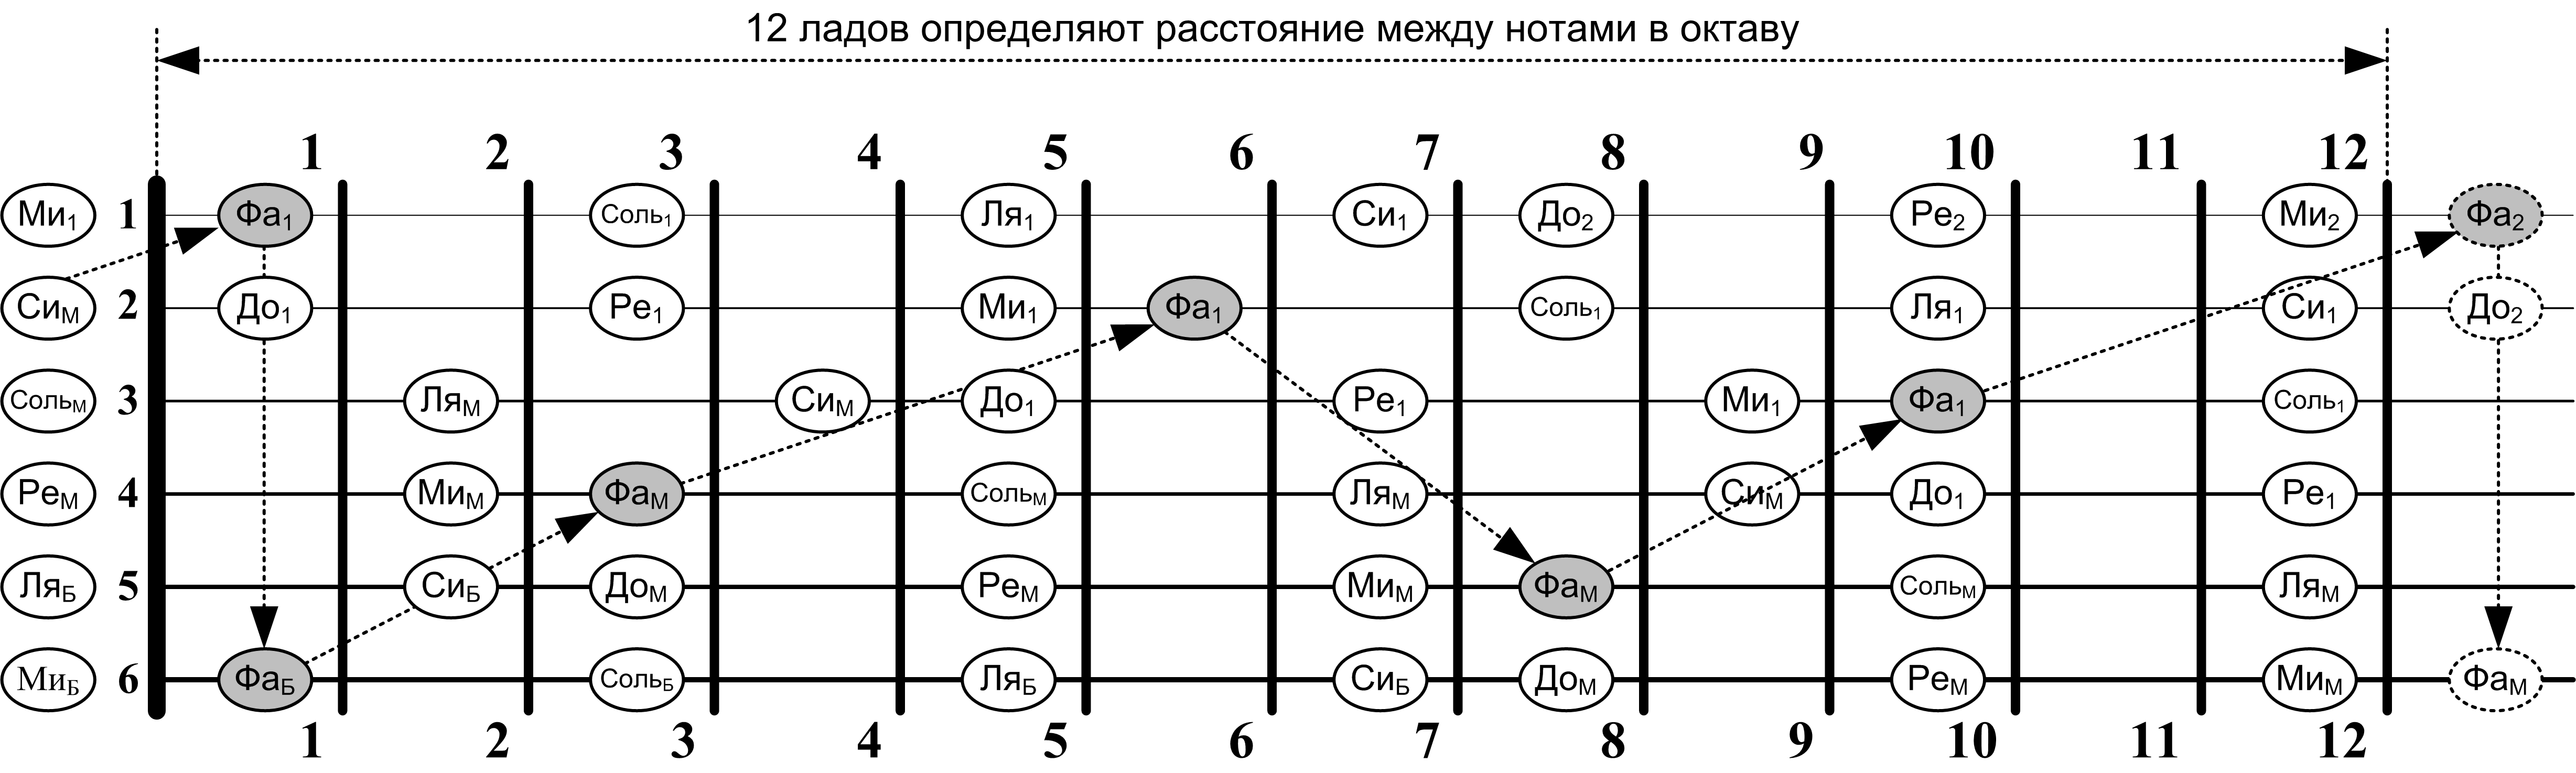
\includegraphics[width=\textwidth]{fig/notes-on-griph} 
    \caption{Ноты на грифе (относительное расположение)}\label{fig:guitar:notes-on-griph}
\end{figure} 


